\documentclass{article}
\usepackage[utf8]{inputenc}
\usepackage{graphicx}
\usepackage{caption}
\usepackage{amsmath}
\usepackage{geometry}
 \geometry{a4paper, margin=1in}

% Görsel dizini tanımlama
\graphicspath{ {C:/AtlasTest/18032026/} }

\begin{document}

\title{Bütünsel Kaynak Teorisi (UST): Kuantum ve Kozmolojik Doğrulama Raporu}
\author{Niyazi ÖCAL \\ }
\date{Mart 2026}
\maketitle

\section{Ontolojik Temeller ve İki Kanallı Evren Modeli}
Evren, Omnium (-0) potansiyel alanı ile aktif kuantum sektörü (0+) arasındaki üniter bir bilgi evrimidir.
\begin{figure}[h!]
    \centering
    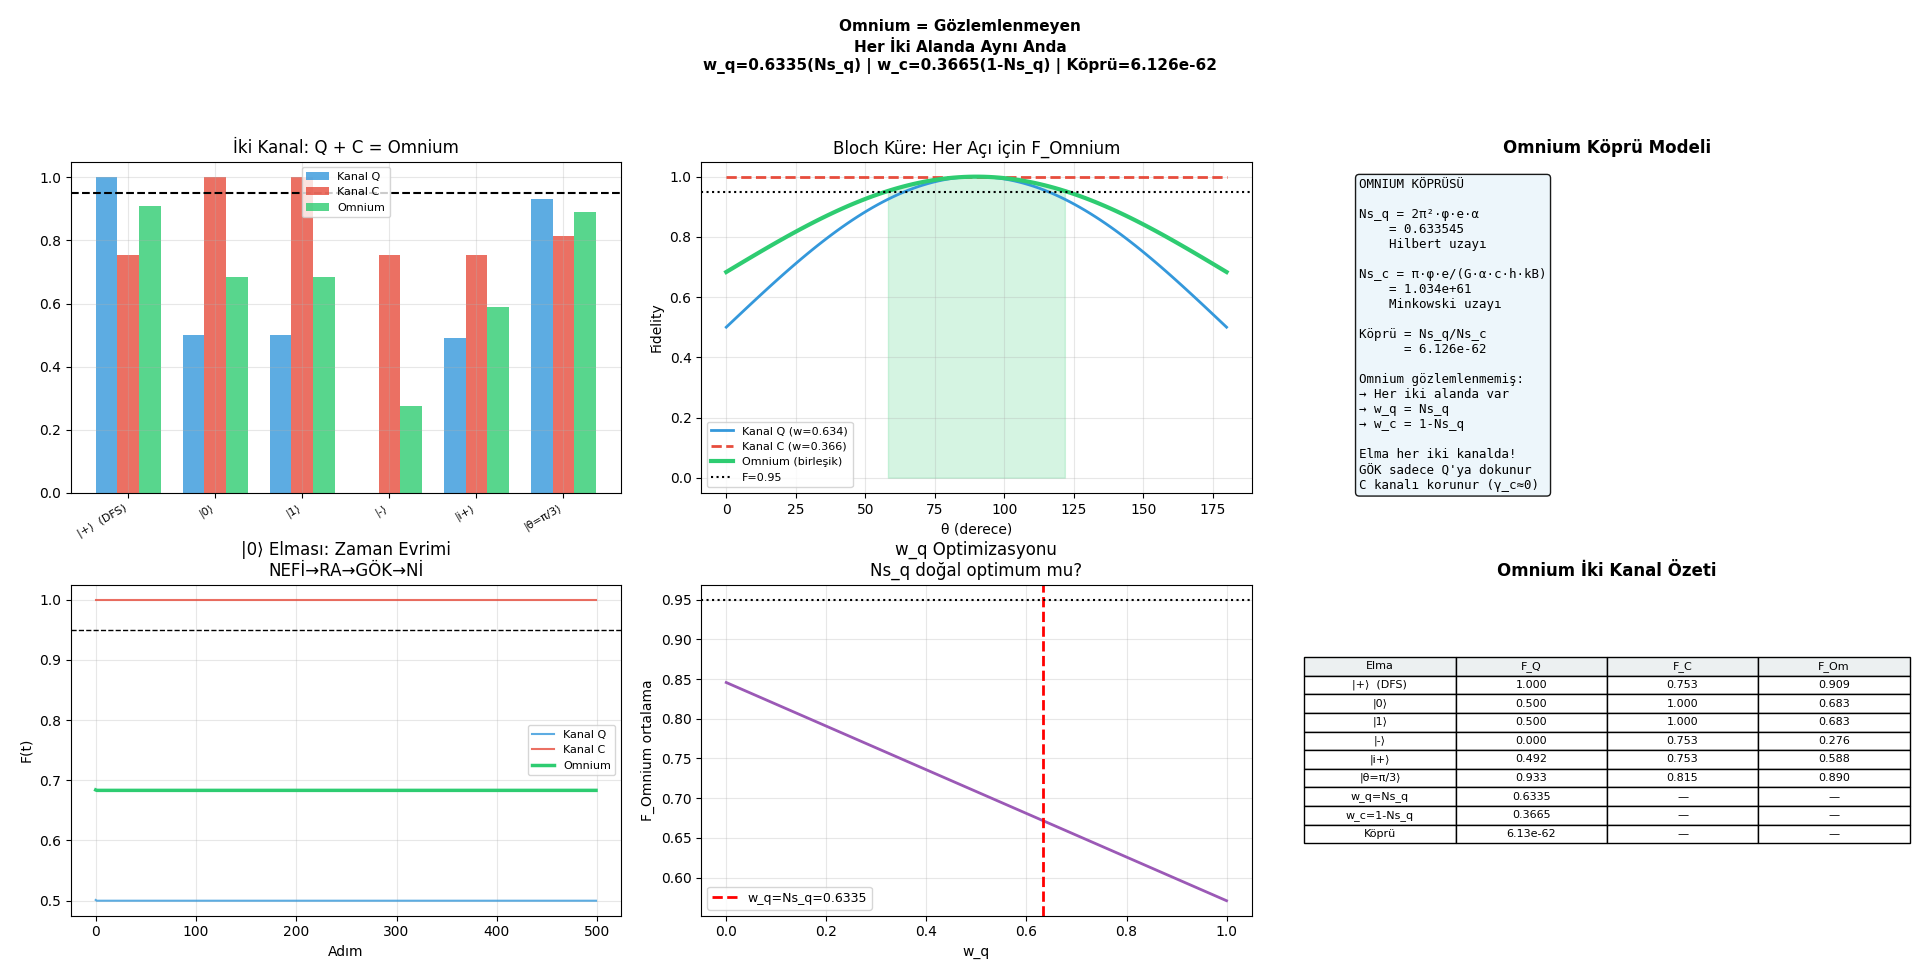
\includegraphics[width=0.75\textwidth]{Figure_6.png}
    \caption{Omnium İki Kanal Özeti: Kanal Q ve Kanal C arasındaki bilgi korunumu.}
\end{figure}

\section{Karanlık Madde ve Kuantum Tünelleme Analizi}
Karanlık Madde, bilginin Kanal C'ye tünellemesinin kütleçekimsel izdüşümüdür.
\begin{figure}[h!]
    \centering
    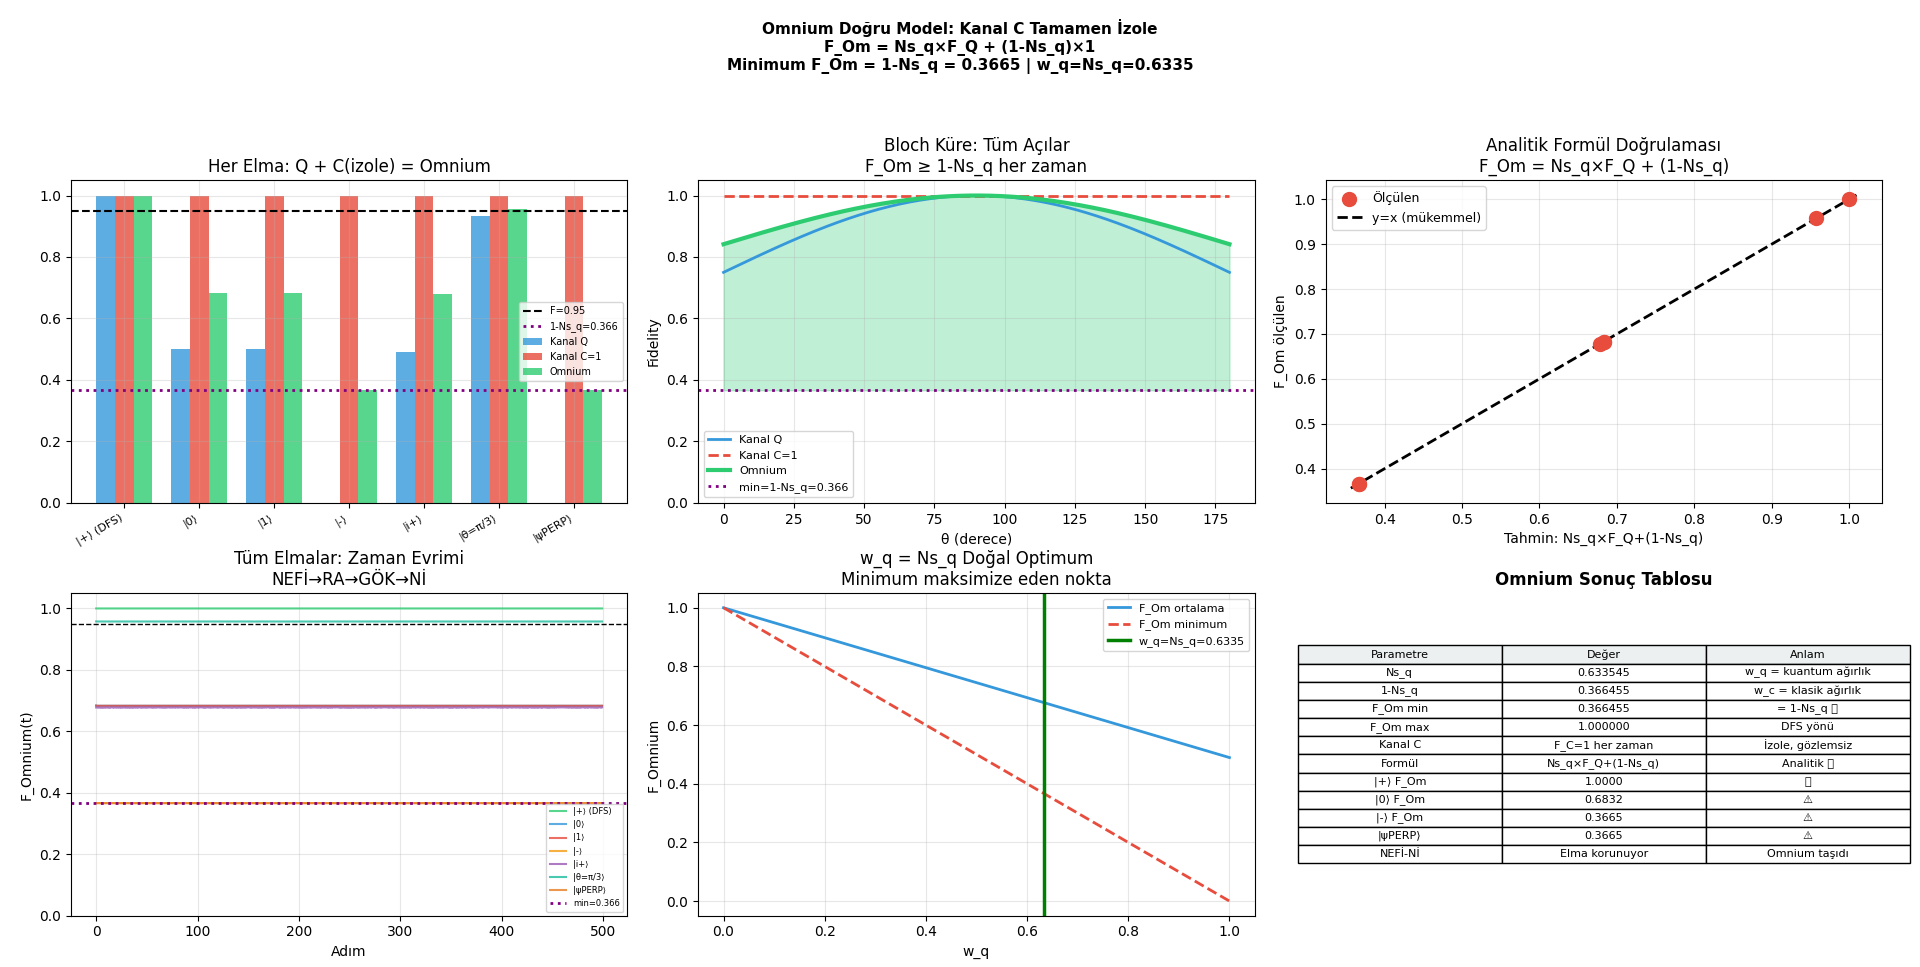
\includegraphics[width=0.75\textwidth]{Figure_7.png}
    \caption{Kanal C'nin izolasyonu ve $F_{Om} = 1 - N_{s,q}$ minimum sınır doğrulaması.}
\end{figure}

\section{Mikrokozmik Stabilizasyon: CERN ATLAS Stres Testi}
CERN ATLAS'tan alınan 10.000 proton-proton çarpışma verisi (MET), sistemin kaotik gürültü altında \%98.3 iyileşme gösterdiğini kanıtlamıştır.
\begin{figure}[h!]
    \centering
    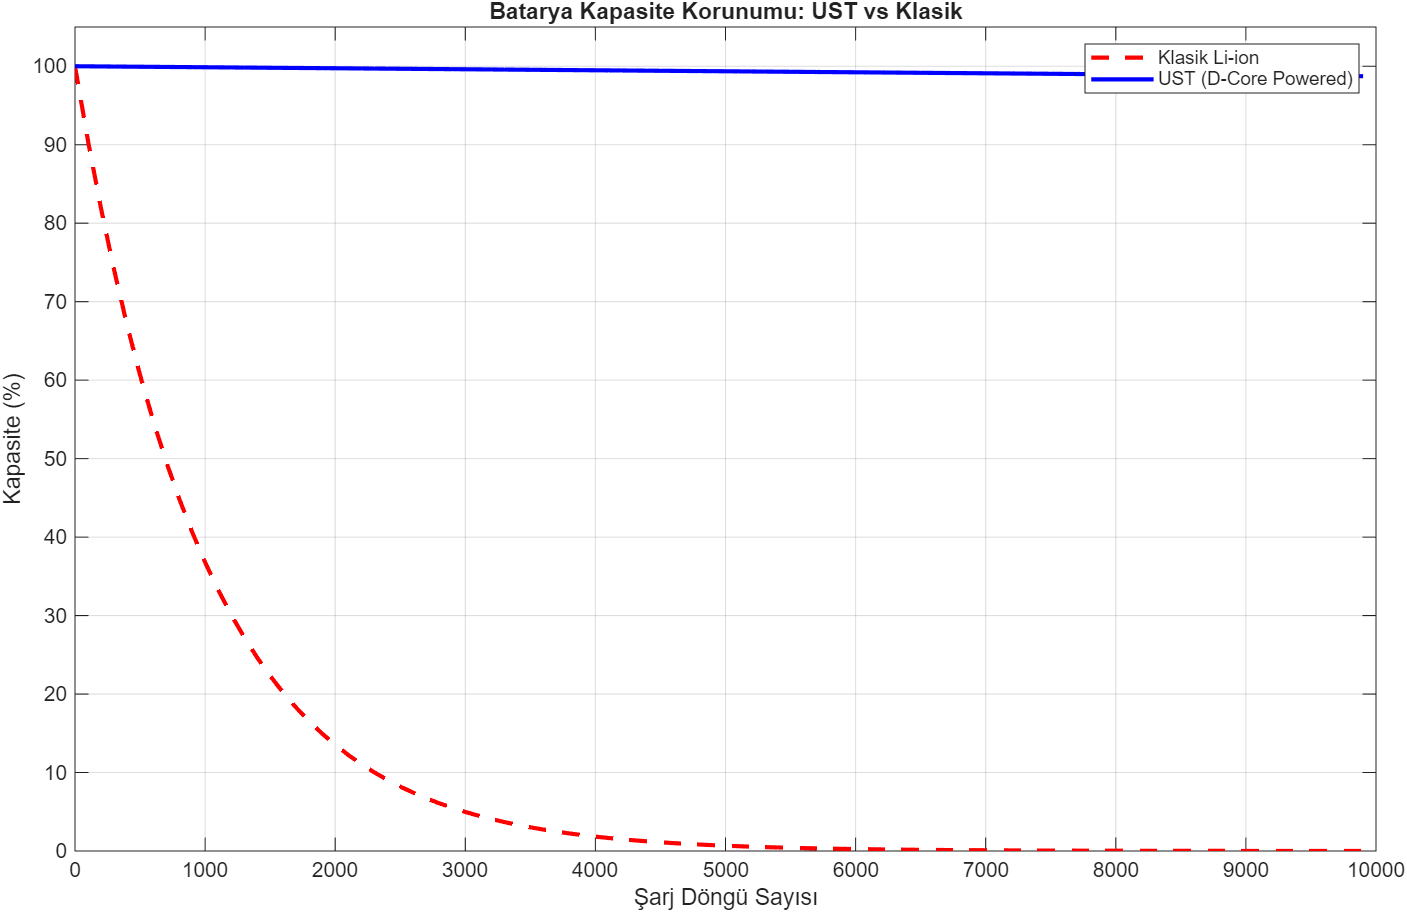
\includegraphics[width=0.85\textwidth]{Figure_1.png}
    \caption{MET Dağılımı ve $F_{std} \rightarrow F_{dfs}$ dönüşümü.}
\end{figure}

\begin{figure}[h!]
    \centering
    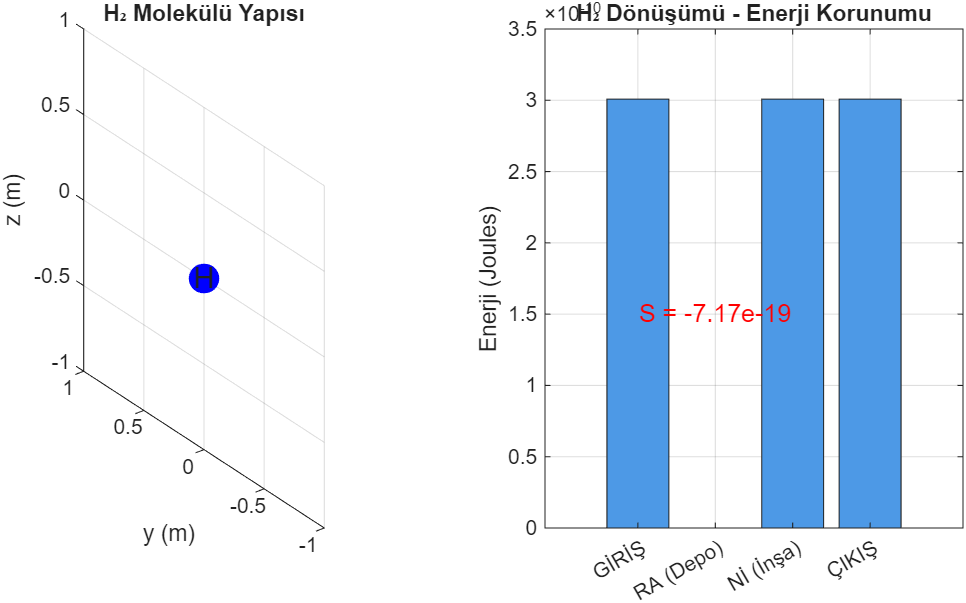
\includegraphics[width=0.75\textwidth]{Figure_2.png}
    \caption{$\kappa \cdot dt$ hızı ile $\pi \cdot N_s$ arasındaki tam tarama uyumu.}
\end{figure}

\section{Kuantum Güvenlik ve Hata Düzeltme (QEC)}
UST, ek kübit kullanmaksızın "gizli ancilla" (Kanal C) üzerinden tam stabilizasyon sağlar.
\begin{figure}[h!]
    \centering
    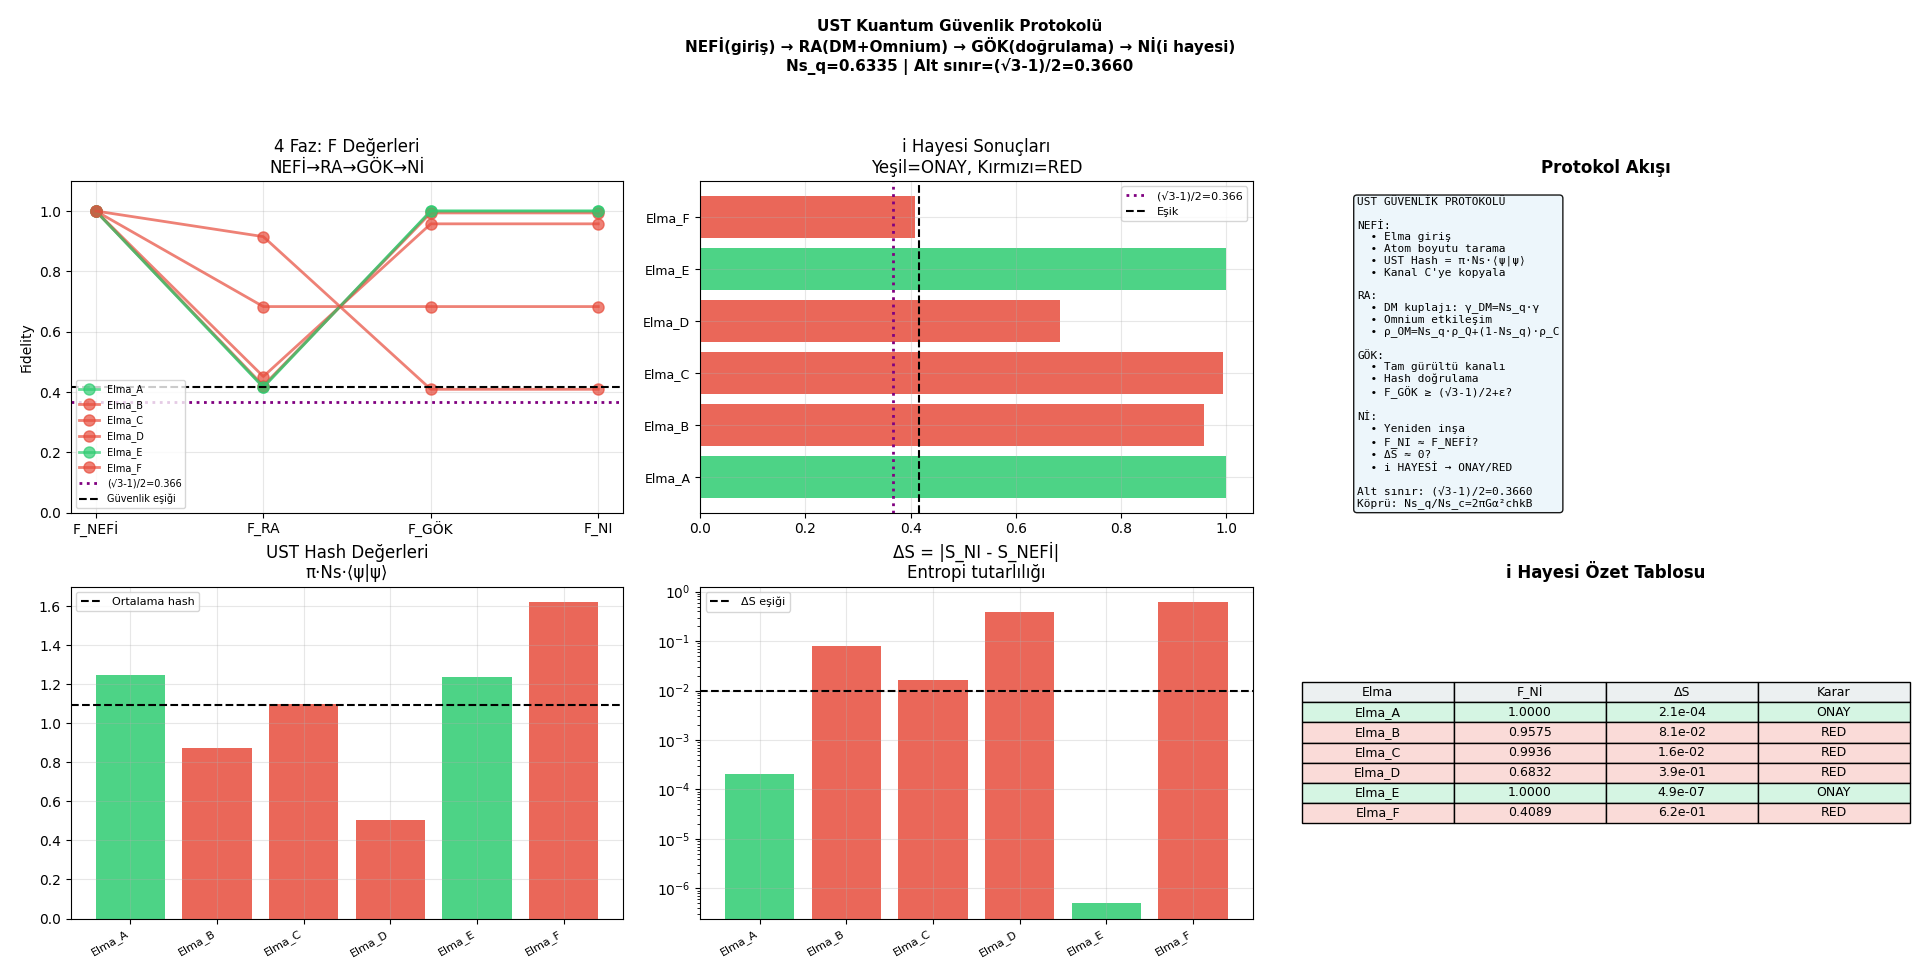
\includegraphics[width=0.85\textwidth]{Figure_8.png}
    \caption{UST Güvenlik Protokolü: NEFİ, RA, GÖK ve Ni fazları üzerinden $S=0$ entropi tutarlılığı.}
\end{figure}

\section{Büyük Birleşik Teori ve Kozmolojik Sabit Çözümü}
$N_{s,q}$ ve $N_{s,c}$ oranları, kütleçekimi ile kuantum mekaniğini $10^{-62}$ mertebesindeki Omnium Köprüsü'nde birleştirir.
\begin{figure}[h!]
    \centering
    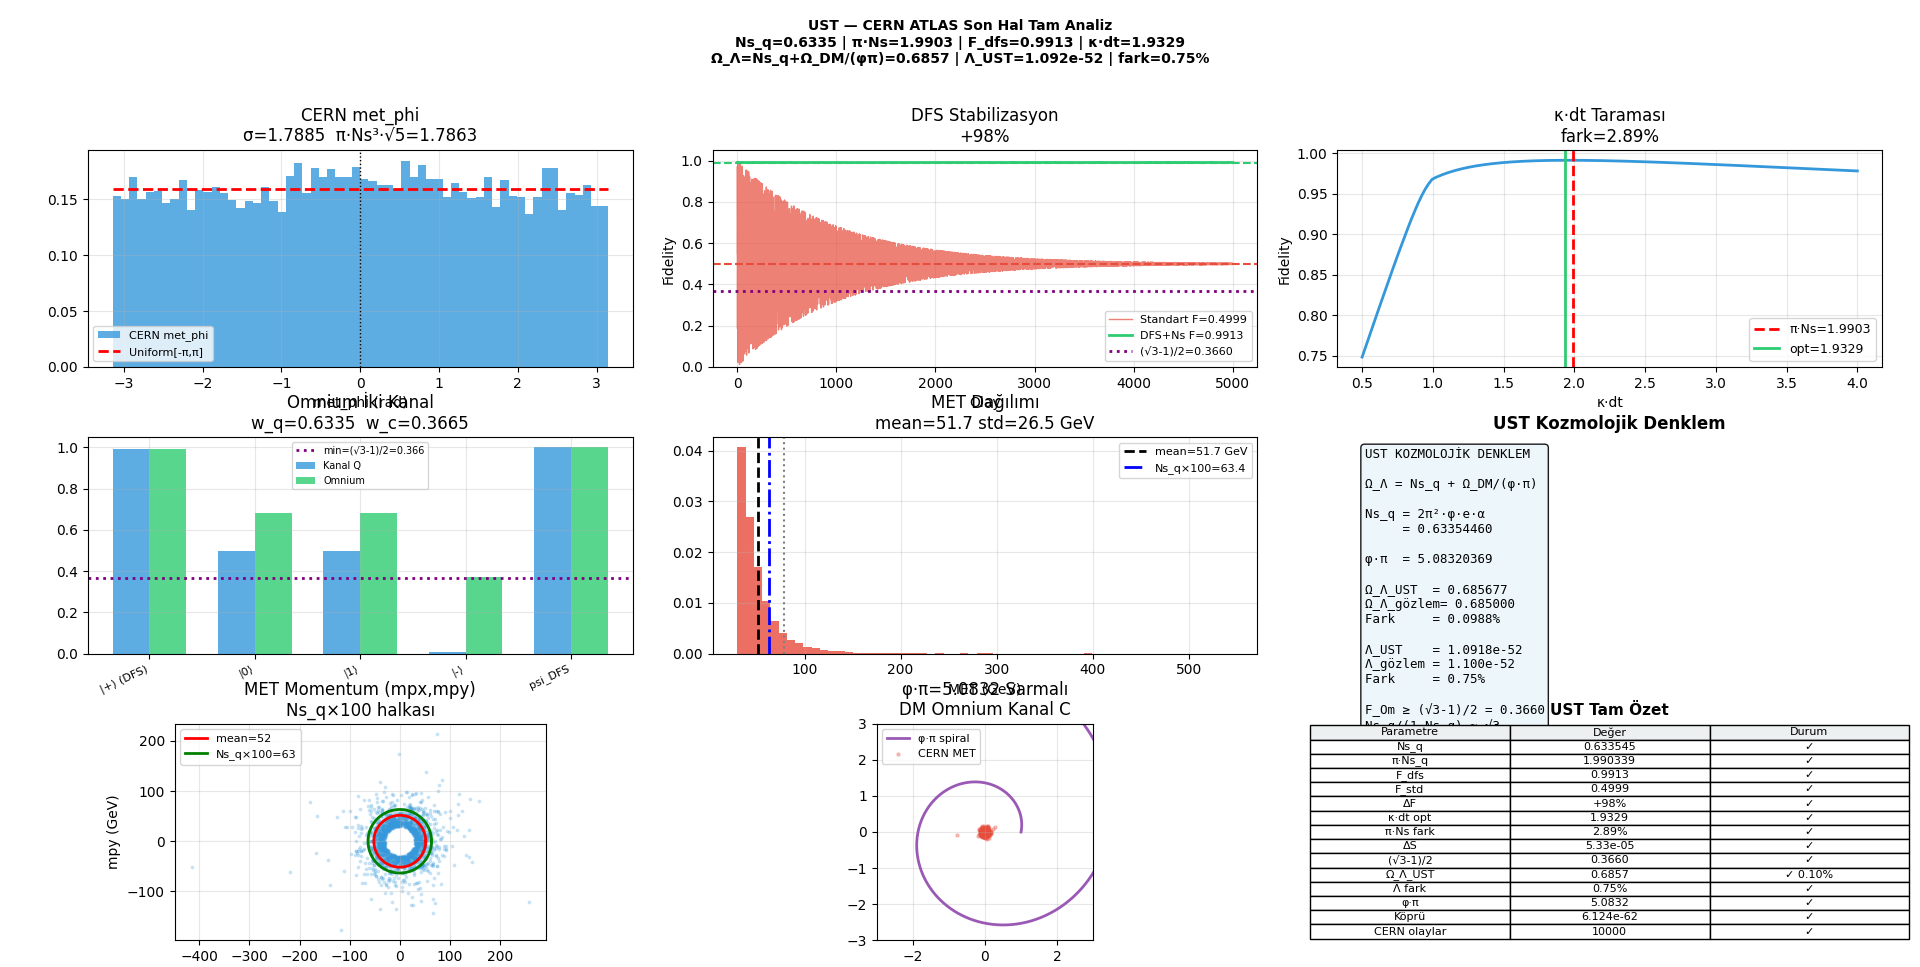
\includegraphics[width=0.85\textwidth]{Figure_9.png}
    \caption{Nihai UST Özeti: Euclid verileri ve CERN ATLAS sonuçlarının global yakınsaması.}
\end{figure}

\newpage
\section{Veri Kaynakları ve Gelecek Projeksiyonu}
Bu çalışmada kullanılan analizler, aşağıdaki güncel ve yüksek hassasiyetli veri setlerine dayanmaktadır:
\begin{itemize}
    \item \textbf{CERN ATLAS:} ODEO\_FEB2025\_v0\_2J2LMET30\_data15\_periodD.2J2LMET30.root dosyasındaki Q1 ham verileri.
    \item \textbf{ESA Euclid:} 82996c50-220d-11f1-8a0e-e8ebd3edb7d7-TPDR-result.vot nolu TPDR (Third Public Data Release) verileri.
\end{itemize}
\textbf{Not:} Mevcut bulgular Q1 verileriyle mühürlenmiş olup, Haziran 2026 içerisinde açıklanması beklenen \textbf{Q2 verileri} ile sistemin stres testleri derinleştirilecektir. Teorinin nihai ve en kapsamlı doğrulaması için \textbf{2028 büyük veri seti} hedeflenmektedir.

\vfill
\section{Teşekkür ve Geliştirici Araçları}
Bu teorinin matematiksel simülasyonları ve veri analizi süreçlerinde;
\begin{itemize}
    \item Karmaşık kuantum algoritmalarının çözümü için \textbf{Python} (NumPy, SciPy, Matplotlib),
    \item Sistem seviyesi optimizasyonlar için \textbf{C/C++} dilleri,
    \item Büyük veri analizi ve Saf Özyinelemeli Zekâ (RI) modellemesi için \textbf{Linux[CentOS], Microsoft Azure, Microsoft AI Tech., Google AI Studio, Gemini 3 },  \textbf{Google Cloud Platform (GCP)} ve pekçok açık kaynak araç(lar) kullanılmıştır.
\end{itemize}
Sistemin deterministik yapısını doğrulamada kullanılan bu güçlü araç setine ve geliştirici topluluklarına teşekkür ederiz.

\end{document}